\documentclass[runningheads,a4paper]{llncs}
\newcommand*{\rootPath}{./}

\usepackage{url}
\usepackage[utf8]{inputenc}
\newcommand{\inlinecode}{\texttt}
\usepackage{microtype}
% \usepackage[colorlinks]{hyperref}

% math and cs
% \usepackage[lined,boxed,commentsnumbered]{algorithm2e}
% \usepackage{amsmath}
% \usepackage{amssymb}
% \usepackage{mathrsfs}

% style
% \usepackage{booktabs}
% \usepackage{multirow}
\usepackage{listings} % code highlighting
\lstset{language=C++,
                basicstyle=\ttfamily,
                keywordstyle=\color{blue}\ttfamily,
                stringstyle=\color{red}\ttfamily,
                commentstyle=\color{green}\ttfamily,
                morecomment=[l][\color{magenta}]{\#}
}
\usepackage{todonotes}
\usepackage{standalone}


% graph
\usepackage{graphicx}
\usepackage[outdir=./]{epstopdf}
\usepackage{array}



% \usepackage[french]{babel}
\usepackage[nomain,acronym,xindy,toc]{glossaries}
\makeglossaries
\usepackage[xindy]{imakeidx}
\makeindex




% questions
\newcounter{question}
\newcommand\Que[1]{%
    \bfseries
   \leavevmode\par
   \stepcounter{question}
   \noindent
   Q  --- #1\par\mdseries}


% reponses
\def\showanswers{1}% Set this =0 to hide, =1 to show
\newcommand\Ans[2][]{%
    \ifnum\showanswers=1
        \bfseries
        \leavevmode\par\noindent
       {\leftskip37pt
        R --- \textbf{#1}#2\par}\mdseries
    \fi
}


\newcommand\darwin{\texttt darwin-op}











\newglossaryentry{firmware}{
    name={firmware},
    description={programme intégré dans un matériel informatique (ordinateur, photocopieur, automate (API, APS), disque dur, routeur, appareil photo numérique, etc.) pour qu'il puisse fonctionne}
}


\newglossaryentry{framework}{
    name={framework},
    description={ensemble cohérent de composants logiciels structurels, qui sert à créer les fondations ainsi que les grandes lignes de tout ou d’une partie d'un logiciel (architecture)}
}
\newglossaryentry{instance}{
    name={instance},
    description={objet constituant un exemplaire de la classe}
}

%\newcolumntype{C}[1]{>{\centering}m{#1}}
%\newcolumntype{C}[1]{>{\centering\raggedright\arraybackslash}m{#1}}
\newcolumntype{L}[1]{>{\raggedright\let\newline\\\arraybackslash\hspace{0pt}}m{#1}}
\newcolumntype{C}[1]{>{\centering\let\newline\\\arraybackslash\hspace{0pt}}m{#1}}
\newcolumntype{R}[1]{>{\raggedleft\let\newline\\\arraybackslash\hspace{0pt}}m{#1}}

\standalonetrue

\title{TP C++ : gestion des classes abstraites dans Darwin-Op}
\titlerunning{TP C++}

\author{Pierre-Louis Guhur,  \inst{1}
        Thomas Rodet \inst{1}}
\authorrunning{Guhur et Rodet}
\institute{
ENS Paris-Saclay (France)
}


\makeglossaries

\begin{document}





\maketitle

\begin{abstract}
C++ est un langage de programmation qui est compilé, avec une large variété de plateformes le supportant.
Il implémente différentes paradigmes, comme la programmation procédurale  la programmation orientée objet, et la programmation générique.
C'est l'un des langages les plus populaires, et est disponible sur la plupart des plateformes.
L'objectif de ce TP est de visiter certains concepts propres à ce langage.
On s'appliquera sur une application réelle : le robot Darwin-Op.
Ainsi, à la fin du TP, on pourra programmmer une séquence de mouvements.
\end{abstract}



% \newacronym{ddye}{D$_{\text{dye}}$}{donor dye, ex. Alexa 488}
% \newacronym[description={\glslink{r0}{F\"{o}rster distance}}]{R0}{$R_{0}$}{F\"{o}rster distance}
% \newglossaryentry{r0}{name=\glslink{R0}{\ensuremath{R_{0}}},text=F\"{o}rster distance,description={F\"{o}rster distance, where 50\% ...}, sort=R}
% \newglossaryentry{kdeac}{name=\glslink{R0}{\ensuremath{k_{DEAC}}},text=$k_{DEAC}$, description={is the rate of deactivation from ... and emission)}, sort=k}


\newglossaryentry{firmware}{
    name={firmware},
    description={programme intégré dans un matériel informatique (ordinateur, photocopieur, automate (API, APS), disque dur, routeur, appareil photo numérique, etc.) pour qu'il puisse fonctionne}
}


\newglossaryentry{framework}{
    name={framework},
    description={ensemble cohérent de composants logiciels structurels, qui sert à créer les fondations ainsi que les grandes lignes de tout ou d’une partie d'un logiciel (architecture)}
}
\newglossaryentry{instance}{
    name={instance},
    description={objet constituant un exemplaire de la classe}
}


\documentclass[conference]{IEEEtran}
\newcommand*{\rootPath}{../}
\usepackage{url}
\usepackage[utf8]{inputenc}
\newcommand{\inlinecode}{\texttt}
\usepackage{microtype}
% \usepackage[colorlinks]{hyperref}

% math and cs
% \usepackage[lined,boxed,commentsnumbered]{algorithm2e}
% \usepackage{amsmath}
% \usepackage{amssymb}
% \usepackage{mathrsfs}

% style
% \usepackage{booktabs}
% \usepackage{multirow}
\usepackage{listings} % code highlighting
\lstset{language=C++,
                basicstyle=\ttfamily,
                keywordstyle=\color{blue}\ttfamily,
                stringstyle=\color{red}\ttfamily,
                commentstyle=\color{green}\ttfamily,
                morecomment=[l][\color{magenta}]{\#}
}
\usepackage{todonotes}
\usepackage{standalone}


% graph
\usepackage{graphicx}
\usepackage[outdir=./]{epstopdf}
\usepackage{array}



% \usepackage[french]{babel}
\usepackage[nomain,acronym,xindy,toc]{glossaries}
\makeglossaries
\usepackage[xindy]{imakeidx}
\makeindex




% questions
\newcounter{question}
\newcommand\Que[1]{%
    \bfseries
   \leavevmode\par
   \stepcounter{question}
   \noindent
   Q  --- #1\par\mdseries}


% reponses
\def\showanswers{1}% Set this =0 to hide, =1 to show
\newcommand\Ans[2][]{%
    \ifnum\showanswers=1
        \bfseries
        \leavevmode\par\noindent
       {\leftskip37pt
        R --- \textbf{#1}#2\par}\mdseries
    \fi
}


\newcommand\darwin{\texttt darwin-op}











\newglossaryentry{firmware}{
    name={firmware},
    description={programme intégré dans un matériel informatique (ordinateur, photocopieur, automate (API, APS), disque dur, routeur, appareil photo numérique, etc.) pour qu'il puisse fonctionne}
}


\newglossaryentry{framework}{
    name={framework},
    description={ensemble cohérent de composants logiciels structurels, qui sert à créer les fondations ainsi que les grandes lignes de tout ou d’une partie d'un logiciel (architecture)}
}
\newglossaryentry{instance}{
    name={instance},
    description={objet constituant un exemplaire de la classe}
}


\standalonetrue

\begin{document}

%%=============================================================================



%%=============================================================================
%-------------------------------------------------------------------------------
%   INTRODUCTION
%-------------------------------------------------------------------------------

\section{Introduction}
\label{sec:intro}


Chaque langage de programmation développe une propre philosophie, et chaque philosophie peut être appréhendée par les paradigmes de programmation.

Décrite par son fondateur Bjarne Stroustrup \cite{stroustrup}, la philosophie du C++ propose entre autres de :
\begin{itemize}
    \item laisser le choix d'un style de programmation aux développeurs ;
    \item apporter les options utiles est plus important que de veiller à ce qu'elle soit mal utilisée ;
    \item organiser les programmes de manière séparés et bien définies.
\end{itemize}
Cela signifie que le développeur a une grande liberté dans son utilisation du langage. Pour éviter de produire un code difficile à relire ou à étendre \cite{stroustrup2}, le développeur doit donc comprendre les paradigmes utilisés.

Le C++ utilise la programmation orientée objet et générique. C'est une extension de la programmation procédurale (utilisée en C par exemple). Dans cette dernière, des fonctions sont utilisées, ce qui permet d'éviter des redondances de code et de mettre en place des algorithmes récursifs.
La programmation orientée objet et générique utilise les notions de classes et de modèles pour mutualiser et unifier les informations entre différentes entitées.


Ce travail pratique va explorer ces notions au travers d'exemples de difficultés progressives sur le robot darwin-ops.
Dans une première partie, le robot darwin-op et son framework sont explorés.
Dans une seconde partie, un module de mouvement (MotionModule) est intégré.

Le texte du TP et le code utilisé sont dispobles sur le répertoire git \cite{git}. En cas d'erreurs ou de mises-à-jour, merci de lancer un pull-request.

\end{document}

\documentclass[conference]{IEEEtran}
\newcommand*{\rootPath}{../}
\usepackage{url}
\usepackage[utf8]{inputenc}
\newcommand{\inlinecode}{\texttt}
\usepackage{microtype}
% \usepackage[colorlinks]{hyperref}

% math and cs
% \usepackage[lined,boxed,commentsnumbered]{algorithm2e}
% \usepackage{amsmath}
% \usepackage{amssymb}
% \usepackage{mathrsfs}

% style
% \usepackage{booktabs}
% \usepackage{multirow}
\usepackage{listings} % code highlighting
\lstset{language=C++,
                basicstyle=\ttfamily,
                keywordstyle=\color{blue}\ttfamily,
                stringstyle=\color{red}\ttfamily,
                commentstyle=\color{green}\ttfamily,
                morecomment=[l][\color{magenta}]{\#}
}
\usepackage{todonotes}
\usepackage{standalone}


% graph
\usepackage{graphicx}
\usepackage[outdir=./]{epstopdf}
\usepackage{array}



% \usepackage[french]{babel}
\usepackage[nomain,acronym,xindy,toc]{glossaries}
\makeglossaries
\usepackage[xindy]{imakeidx}
\makeindex




% questions
\newcounter{question}
\newcommand\Que[1]{%
    \bfseries
   \leavevmode\par
   \stepcounter{question}
   \noindent
   Q  --- #1\par\mdseries}


% reponses
\def\showanswers{1}% Set this =0 to hide, =1 to show
\newcommand\Ans[2][]{%
    \ifnum\showanswers=1
        \bfseries
        \leavevmode\par\noindent
       {\leftskip37pt
        R --- \textbf{#1}#2\par}\mdseries
    \fi
}


\newcommand\darwin{\texttt darwin-op}











\newglossaryentry{firmware}{
    name={firmware},
    description={programme intégré dans un matériel informatique (ordinateur, photocopieur, automate (API, APS), disque dur, routeur, appareil photo numérique, etc.) pour qu'il puisse fonctionne}
}


\newglossaryentry{framework}{
    name={framework},
    description={ensemble cohérent de composants logiciels structurels, qui sert à créer les fondations ainsi que les grandes lignes de tout ou d’une partie d'un logiciel (architecture)}
}
\newglossaryentry{instance}{
    name={instance},
    description={objet constituant un exemplaire de la classe}
}


\standalonetrue

\begin{document}
\lstset{language=C++}
%%=============================================================================



%%=============================================================================
%-------------------------------------------------------------------------------
%   EXPLORATION DE DARWIN-OP
%-------------------------------------------------------------------------------

\section{Exploration du robot Darwin-Op}
\label{sec:exploration}

Le robot darwin-op repose sur un cœur Linux et un \gls{framework} développé spécialement pour lui. L'objectif de cette partie est de prendre connaissances du robot, puis de tracer son architecture et le diagramme de classes de son framework. Enfin, nous chercherons à justifier certains choix de conception.


\subsection{Présentation du robot}

Darwin-op est l'acronume de "Dynamic Anthropomorphic Robot with Intelligence–Open Platform". C'est un robot humanoïde miniature (45 cm pour 2.9 kg), capable de marcher (environ 30 cm/s), de se relever (environ 3s), équipé d'une grande capacité de calculs (1.6 GHz Intel Atom Z530 (32 bit) et 4 GB flash SSD), de capteurs avancées (caméra, gyroscope 3 axes, accéléromètre 3 axes, 2 microphones). Il a été développé et construit par l'industriel coréen ROBOTIS en collaboration avec Virginia Tech, Purdue University et l'University of Pennsylvania. DARWIN-OP a 22 degrées de libertés (6 pour chaque jambe, 5 pour chaque bras, 2 pour le cou) contrôlées par des servo-moteurs DYNAMIXEL MX-28T. Le MX-28T a un couple de 24 kgf·cm (à 12 V, 1.5 A) et un déplacement angulaire de 360 degrées.


\subsection{Connexion au robot}

Le robot peut être interfacé de différentes manières :
\begin{itemize}
    \item  par Ethernet avec un câble RJ45 :
    configurer son adresse IP en 192.168.123.100 et le masque de réseau en 255.255.255.0.
    L'adresse du robot est 192.168.123.1.
    Ou bien,  connecter le cable Ethernet au réseau local de la salle.
    \item  par Wi-Fi : un compte Cr@ns est disponible (darwin-op et pi5vrb75uu).
\end{itemize}

Une fois reliée, la communication peut se faire par une connexion série (en utilisant Minicom ou PuTTY par exemple), ou SSH. Dans ce dernier cas, on lancera la commande
    \inlinecode{ssh -X darwin@darwin.peea.ens-cachan.fr} suivie du mot de passe 111111.
    Passer en root avec \inlinecode{sudo -s}.

Si on connecte le robot à un écran (un port HDMI le permet), on pensera à redémarrer le robot.


\subsection{Découverte de l'architecture}

La commande \inlinecode{tree} permet de tracer l'arbre hiérarchique des fichiers dans un répertoire. L'option "-L" limite le nombre de niveaux à visualiser

\Que{ Tracez l'arbre des dossiers à la racine du système de fichiers avec 2 niveaux. Que remarquez-vous de particulier par rapport à un système Linux classique ?}
Il se peut que tree ne soit pas installé par défaut. On peut l'installer avec la commande : \inlinecode{apt-get install tree}.

\Ans{On doit remarquer que le dossier /darwin existe et préciser son contenu (Data = données de mouvements et de sons, Framework = classes utilisées par le robot, Linux = interface entre les composants). Si le code n'existe pas, on peut le réinstaller depuis le répertoire Git.}

Le dossier darwin contient l'ensemble des programmes propres au robot, et en particulier, il permet d'interfacer les composants matériels propres à darwin-op, avec en particulier le sous-contrôleur CM730, qui réalise les tâches en temps réel.

Différents projets sont proposés par le fabriquant dans le dossier \inlinecode{Linux/project}. Nous allons tester \inlinecode{demo}.

\Que{Compilez le code et lancez son éxecution. Le robot doit suivre une balle rouge présentée sous ses yeux.}

\Ans{On se déplace dans le dossier : \inlinecode{cd /darwin/Linux/project/demo},  on compile : \inlinecode{make}, on change les droits d'éxecution : \inlinecode{chmod u+x demo}, puis on éxecute le programme : \inlinecode{./demo}}

Nous allons désormais visiter le code correspondant pour comprendre les initialisations réalisées.

\Que{Ouvrez le fichier \inlinecode{main.cpp} avec un éditeur de texte, puis relevez quelques \gls{instance}s de classe. À votre avis, à quoi correspondent-elles ? Pourquoi certaines utilisent le mot \inlinecode{new} ? }

\Ans{Quelques instances.
\begin{itemize}
    \item \lstinline{minIni* ini = new minIni(INI_FILE_PATH);} parse le fichier de configuration.
    \item \lstinline{$Image* rgb_output = new Image(Camera::WIDTH, Camera::HEIGHT, Image::RGB_PIXEL_SIZE);$} créé une nouvelle image. Il est intéressant de noter que l'on utilise un attribut statique de cette même classe \lstinline{Image::RGB_PIXEL_SIZE}.
\end{itemize}
Le mot clé new alloue de la mémoire dans l'espace libre. Il faut donc écrire un delete pour le supprimer. On obtient alors un pointeur vers l'objet. Sans le mot new, l'allocation est directement dans la pile et l'objet est détruit en sortant de la zone de code correspondante.}

Différentes classes du framework sont ici employées. Nous allons désormais les explorer à l'aide d'un diagramme de classes.
Pour tracer un diagramme de classes, on peut utiliser MagicDraw : on créé un nouveau projet "Software Engineering" : "Project from Existing Source Code", puis on sélectionne tous les fichiers concernés, et on clique droit pour générer le diagramme.

\Que{Tracer le diagramme de classes pour \inlinecode{Head}, \inlinecode{MotionModule}, \inlinecode{Walking} et \inlinecode{Action}. Quelles sont les relations entre ces classes ?}

\Ans{Relation de généralisation : les classes héritent de MotionModule. Relation d'agrégation : les classes de type
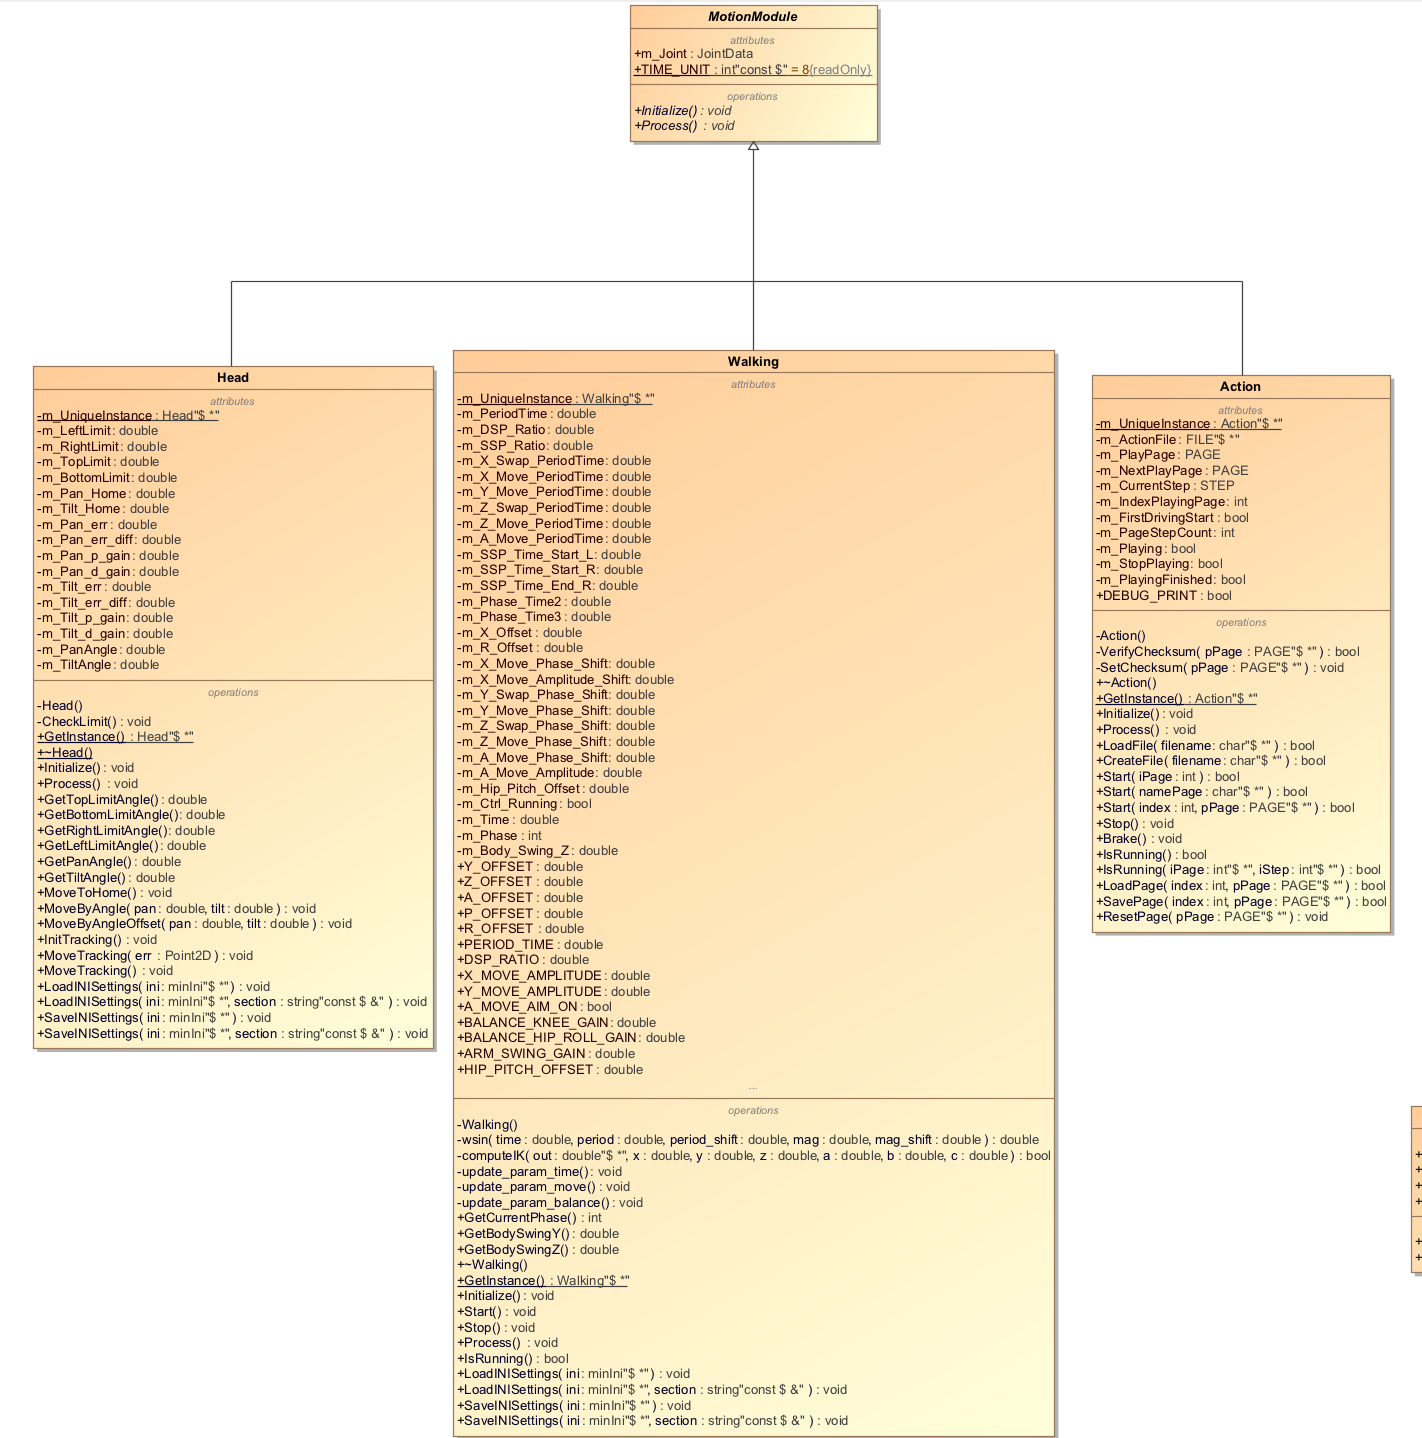
\includegraphics{diagramme-classes.png}}



\subsection{Notion de généricité}

La notion de généricité définit des objets paramétrés par le type qu'ils manipulent. Nous allons voir que la classe ModuleManager peut manier indifféremment les classes Head, Walking et Action.

Un objet générique n'est alors pas directement utilisable : c'est plutôt un patron de module qui sera instancié par les types paramètres qu'il accepte.


\Que{Ouvrez les fichiers \inlinecode{Framework/src/motion/MotionManager.cpp} et \inlinecode{Framework/include/MotionManager.h}. Quelle est la relation entre la classe MotionManager et MotionModule ?}


\Ans{Relation d'agrégation : les classes de type MotionModule peuvent facultativement être ajoutées à la liste \lstinline{std::list<MotionModule*> m_Modules;} }

\subsubsection{Containeur}
L'attribut \lstinline{m_Modules} est en fait un containeur. Il permet de stocker des objets de n'importe quel type (celui en paramètre de la liste), à partir du moment où la classe correspondante est dotée d'un certain nombre de méthodes nécessaires à la librairie \inlinecode{stl} (pour une classe X) :
\begin{itemize}
    \item \lstinline{X()} : un constructeur par défaut,
    \item \lstinline{X(const X&)} : un constructeur par copie,
    \item \lstinline{operator=(const X&)} : l'opérateur d'affectation,
    \item \lstinline{operator==(const X&)} : l'opérateur d'égalité,
    \item \lstinline{operator<(const X&)} : l'opérateur inférieur (utile uniquement pour les tris).
\end{itemize}
Cela peut se réaliser grâce au mot-clé "template":
\lstinline{template < class T, class Alloc = allocator<T> > class list;}
\todo{meilleur ex?}

Cependant, cela demande aussi que Head, Walking et Action soient compris comme des classes MotionModule.

\Que{Comment cela est-il possible ? Finalement, pouvez-vous expliquer qu'il n'existe pas de fichiers MotionModule.cpp ? Expliquez la présence du mot clé \lstinline{virtual} dans le fichier \inlinecode{Framework/include/MotionModule.h}. Comment peut-on alors qualifier la classe MotionModule ?}

\Ans{C'est parce que ces classes héritent toutes de MotionModule. Il n'existe pas d'implémentation de MotionModule car on n'utilise que ses classes filles. Le mot clé virtual signifie que la méthode doit être implémentée car les classes filles. La classe est dite abstraite car toutes ses méthodes sont virtuelles.}

 MotionModule est un interface. \todo{approfondir}


\subsubsection{Itérateur}

Dans le fichier MotionModule.cpp, on retrouve les lignes de code suivantes :

\begin{lstlisting}
    for(int id=JointData::ID_R_SHOULDER_PITCH; id<JointData::NUMBER_OF_JOINTS; id++)
    {
        // ...
    }
\end{lstlisting}

\Que{Retrouvez la déclaration de JointData. Comment se fait-il que nous puissions itérer sur cette structure ? Comment \lstinline{NUMBER_OF_JOINTS} peut-il prendre la bonne valeur ?}

\Ans{JointData est défini dans \inlinecode{Framework/include/JointData.h}. Il s'agit d'une structure \lstinline{enum}. À chaque énumérateur, une valeur est associée du type sous-jacent. Par défaut, la première valeur est 0, tandis que les autres valeurs sont égales à la valeur de l'énumérateur précédent incrémenté de 1. En C++ (ce n'est pas le cas en java par exemple), on peut naturellement donc itérer sur les enum. De plus, \lstinline{NUMBER_OF_JOINTS} vaut bien le nombre d'éléments car la liste commence à 1.}

La structure \lstinline{enum} est un cas particulier des itérateurs, lesquels sont une généralisation des pointeurs. Ils permettent au programmeur de travailler avec des containers différents de façon uniforme.

Les containeurs sont souvent dotés d'une méthode begin qui renvoie un itérateur sur le premier de leurs éléments, et d'une méthode end qui renvoie un itérateur sur une place se trouvant juste après le dernier de leurs éléments. Un autre exemple se trouve dans \inlinecode{/Framework/src/motion/MotionManager.cpp} à la ligne 268 :
\begin{lstlisting}
    for(std::list<MotionModule*>::iterator i = m_Modules.begin(); i != m_Modules.end(); i++)
\end{lstlisting}

\subsubsection{Singleton design pattern}

La programmation C++ est si riche de fonctionnalités, que plusieurs modèles de programmation ont émergé pour standardiser les bonnes pratiques.
L'étudiant intrigué pourra se référer au livre "Design Pattern" \cite{gamma1995design} pour en savoir plus.

Le design du singleton garantit qu'une classe est instanciée une seule fois et pas plus. C'est souvent utilisé pour logger des informations, de sorte à éviter des conflits de gestion des ressources. Par exemple :



\begin{lstlisting}
#include <string>

class Logger{

public:
   static Logger* Instance();
   bool openLogFile(std::string logFile);
   void writeToLogFile();
   bool closeLogFile();

private:
   Logger(){};  // on ne peut le construire depuis l'exterieur
   Logger(Logger const&){};
   Logger& operator=(Logger const&){};
   static Logger* m_pInstance; // stocke sa propre instanciation

};
\end{lstlisting}
Dans cette exemple, il est notable que l'instanciation retourne un pointeur vers une variable statique. Seule la méthode Instance peut appeler le constructeur.

\Que{Retrouvez un exemple de ce design dans le Framework.}

\Ans{Par exemple:
\lstinline{MotionManager* MotionManager::m_UniqueInstance = new MotionManager();} }


\subsection{Exercice}

On propose désormais un court exercice pour mettre en œuvre ces notions de généricité.
Le code suivant réalise une liste chaînée.
Une liste chaînée est une structure de données représentant une collection ordonnée et de taille arbitraire d'éléments de même type, dont la représentation en mémoire de l'ordinateur est une succession de nœuds faites d'un contenu et d'un pointeur vers un autre nœud.
De façon imagée, l'ensemble des nœuds ressemble à une chaîne dont les maillons seraient les nœuds.
L'accès aux éléments d'une liste se fait de manière séquentielle : chaque nœud permet l'accès au suivant (contrairement au tableau dans lequel l'accès se fait de manière directe, par adressage de chaque cellule du tableau).


\lstinputlisting[language=C++, firstline=1, lastline=54]{Code/ListeChaineeDebut.cpp}

Différents points sont important de souligner dans cette implémentation :
\begin{itemize}
    \item une classe amie \inlinecode{friend class ListeChainee;} donne accès aux membres privés et protégés à l'amie en question ;
    \item
\end{itemize}

On propose de compléter cette liste chaînée afin d'en faire un itérateur. Il faudra alors ajouter la possibilité d'incrémenter (\inlinecode{i++}) la chaîne.

\Que{Transformez la classe \inlinecode{ListeChainee} en itérateur. Proposez un exemple d'utilisation avec une boucle \inlinecode{for}.}

\Ans{Correction dans le répertoire git \cite{git}.}

La liste chaînée n'accepte que des valeurs entières.

\Que{Modifiez la pour accepter tout type d'objet à l'aide d'un template}

\Ans{Correction dans le répertoire git \cite{git}}

Le cours de David R. Musser \cite{coursLC}  peut compléter cette exercice sur les listes chaînées. Le code proposé est inspiré de celui de cplusplus.com \cite{cplusplus.com}.

\todo{transformer ce TP en notebook}
\end{document}

\documentclass[conference]{IEEEtran}
\newcommand*{\rootPath}{../}
\usepackage{url}
\usepackage[utf8]{inputenc}
\newcommand{\inlinecode}{\texttt}
\usepackage{microtype}
% \usepackage[colorlinks]{hyperref}

% math and cs
% \usepackage[lined,boxed,commentsnumbered]{algorithm2e}
% \usepackage{amsmath}
% \usepackage{amssymb}
% \usepackage{mathrsfs}

% style
% \usepackage{booktabs}
% \usepackage{multirow}
\usepackage{listings} % code highlighting
\lstset{language=C++,
                basicstyle=\ttfamily,
                keywordstyle=\color{blue}\ttfamily,
                stringstyle=\color{red}\ttfamily,
                commentstyle=\color{green}\ttfamily,
                morecomment=[l][\color{magenta}]{\#}
}
\usepackage{todonotes}
\usepackage{standalone}


% graph
\usepackage{graphicx}
\usepackage[outdir=./]{epstopdf}
\usepackage{array}



% \usepackage[french]{babel}
\usepackage[nomain,acronym,xindy,toc]{glossaries}
\makeglossaries
\usepackage[xindy]{imakeidx}
\makeindex




% questions
\newcounter{question}
\newcommand\Que[1]{%
    \bfseries
   \leavevmode\par
   \stepcounter{question}
   \noindent
   Q  --- #1\par\mdseries}


% reponses
\def\showanswers{1}% Set this =0 to hide, =1 to show
\newcommand\Ans[2][]{%
    \ifnum\showanswers=1
        \bfseries
        \leavevmode\par\noindent
       {\leftskip37pt
        R --- \textbf{#1}#2\par}\mdseries
    \fi
}


\newcommand\darwin{\texttt darwin-op}











\newglossaryentry{firmware}{
    name={firmware},
    description={programme intégré dans un matériel informatique (ordinateur, photocopieur, automate (API, APS), disque dur, routeur, appareil photo numérique, etc.) pour qu'il puisse fonctionne}
}


\newglossaryentry{framework}{
    name={framework},
    description={ensemble cohérent de composants logiciels structurels, qui sert à créer les fondations ainsi que les grandes lignes de tout ou d’une partie d'un logiciel (architecture)}
}
\newglossaryentry{instance}{
    name={instance},
    description={objet constituant un exemplaire de la classe}
}


\standalonetrue

\begin{document}

%%=============================================================================



%%=============================================================================
%-------------------------------------------------------------------------------
%   MOUVEMENT
%-------------------------------------------------------------------------------

\section{Recopie du mouvement d'un bras}
\label{sec:intro}

\subsection{Présentation du projet}
Tandis que la partie précédente revisitait les concepts du langage C++, on propose désormais d'écrire un nouveau projet pour le framework \darwin.
Ce dernier va recopier les mouvements imposés au bras droit sur le gras gauche.

Pour faciliter la programmation, on différenciera les fichiers suivants:
\begin{itemize}
    \item Arm.cpp et Arm.h formeront un MotionModule, appelé Arm,
    pour proposer une interface de gestion d'un bras. On placera ces fichiers dans \inlinecode{Framework/src/motion/modules} et \inlinecode{Framework/include}.
    \item  \inlinecode{main.cpp}, situé dans
    \inlinecode{\url{Linux/project/recopier_bras}},
    lancera le programme et éxecutera les méthodes de Arm.
\end{itemize}

\subsection{Classe Arm}

La classe Arm contiendra les attributs et méthodes suivantes :
\begin{itemize}
    % \item GetLeftArm permettra de choisir ces bras ;
    \item AddMotors ;
    \item GetMotorsValues retournera les valeurs des servo-moteurs du bras ;
    \item Scan retournera un tableau avec les positions sur les servo-moteurs ;
    \item Apply prendra en argument un tableau d'ordres sur les servo-moteurs de hardArm et appliquera ces ordres ;
    \item PutSoft et PutHard rendront respectivement le bras mou (on peut imposer manuellement un mouvement) ou dur (on ne peut pas).
\end{itemize}

\Que{Tracez le diagramme de classes de Arm et des objets auxquels Arm se réfère.}

\Ans{\todo{à faire}}

\Que{Programmez \inlinecode{Arm.cpp} et \inlinecode{Arm.h}. Aucun test ne sera pour le moment effectué.}

\Ans{cf. répertoire git.}


\subsection{Projet recopier\_bras}

Ainsi, le fichier main.cpp suivra l'algorithme suivant :
\begin{enumerate}
    \item initialiser le module Arm pour les bras softArm (celui dont on impose manuellement le mouvement) et hardArm (celui qui recopie les mouvements) ;
    \item faire un boucle infini avec :
    \item enregistrer les informations sur softArm ;
    \item appliquer les valeurs sur hardArm.
\end{enumerate}

\Que{Réalisez ce programme. On ne demande pas de compiler le fichier}
\Ans{cf. répertoire git.}

\subsection{Compilation}

Pour compiler le code, on partira d'un Makefile pré-existant, par exemple celui contenu dans \inlinecode{\url{Linux/project/walk_tuner}}.

\Que{Adaptez le Makefile puis lancer la compilation du projet en lançant \inlinecode{make} depuis le dossier du projet. Corrigez d'éventuels erreurs sur le programme puis testez le.}
\Ans{cf. répertoire git.}


\end{document}




\section{Conclusion}
\label{sec:ccl}


Ce TP a permis d'explorer le langage C++ et de se familiariser avec le robot Darwin-Op. En particulier, les concepts suivants ont été vus :
\begin{itemize}
    \item utilisation d'un framework au-dessus d'un système d'exploitation pour programmer un robot (ce qui n'est pas sans rappelé ROS) ;
    \item programmation orienté objet et générique avec les concepts d'héritages, de classes abstraites et de templates ;
    \item l'existance de designs de programmation comme celui du singleton ;
    \item des structures de données comme les containeurs et les listes chaînées.
\end{itemize}
On pourra continuer d'explorer le C++ avec les expressions lambda \cite{lambda}, ou la différence entre le polymorphisme statique et dynamique. La lecture de livres spécialisés est recommandée \cite{gamma1995design}, \cite{jumpingallain}. 




%%=============================================================================
%%=============================================================================
\ifstandalone

    \appendix
    \printglossary[title=Vocabulaire et abbréviations]
	\bibliographystyle{IEEEtran}
	\bibliography{\rootPath Annexes/biblio.bib}
\fi
%%=============================================================================
%%=============================================================================



\end{document}
